% !TEX program = pdflatex
\documentclass[11pt,a4paper]{article}

% ---------- Packages ----------
\usepackage[utf8]{inputenc}
\usepackage[T1]{fontenc}
\usepackage{amsmath,amssymb,amsfonts}
\usepackage{graphicx}
\usepackage{booktabs}
\usepackage{hyperref}
\usepackage{algorithm}
\usepackage{algpseudocode}
\usepackage{listings}
\usepackage{xcolor}
\usepackage{tikz}
\usetikzlibrary{arrows.meta,positioning,shapes.geometric,fit}
\usepackage[margin=2.5cm]{geometry}
\usepackage{natbib}

% ---------- Listings style ----------
\lstset{
  basicstyle=\ttfamily\small,
  keywordstyle=\color{blue}\bfseries,
  commentstyle=\color{gray},
  stringstyle=\color{orange},
  breaklines=true,
  frame=single,
  numbers=left,
  numberstyle=\tiny\color{gray},
}

% ---------- Title ----------
\title{%
  \textbf{MoEx: Distributed Mixture-of-Experts Inference\\
  on Consumer Devices via WebGPU}\\[0.5em]
  \large Browser-Based Expert FFN Disaggregation with\\
  Hedged Dispatch and Binary Transport
}

\author{
  Etzhayyim Research\\
  \texttt{research@etzhayyim.com}\\
  \url{https://web3llm.etzhayyim.com}
}

\date{February 2026}

\begin{document}
\maketitle

% ============================================================
\begin{abstract}
We present \textbf{MoEx} (Mixture-of-Experts Execution), a system for
distributed large language model (LLM) inference that disaggregates
Mixture-of-Experts (MoE) feed-forward network (FFN) computation across
consumer devices---smartphones and browsers---using the WebGPU API.
A centralized \emph{host} runs the attention backbone, KV cache, and
gating router on server-class hardware, while \emph{expert workers}
running on phones execute the selected top-$k$ Expert FFN (SwiGLU)
computations via WebGPU shaders. We design a compact binary protocol
(\textbf{MoEx protocol}, 12-byte header) for low-latency dispatch over
WebSocket, implement speculative hedged execution (50\,ms hedge,
200\,ms resend, 500\,ms fail), and distribute int4-quantized expert
weight sets ($\sim$480\,MB per 4-expert bundle) from object storage.

We target \textbf{Qwen3-30B-A3B} (48 layers, 128 experts, top-4
routing, hidden dim 2048) and describe the decomposition into a
server-side attention/router package and 32 phone-side expert sets.
The system is implemented as a WebAssembly control plane deployed on
SpinKube
with a blobstore provider for model weight distribution, and a
SvelteKit Progressive Web App for the expert worker with WebGPU
compute shaders for GEMM and SiLU$\odot$mul kernels.

We analyze the theoretical latency budget, communication overhead, and
feasibility on current mobile WebGPU implementations (Chrome 121+,
Safari 18+), and discuss the governance model where expert computation
is compensated via on-chain Governance Compute Credits (GCC, ERC-20).
\end{abstract}

\textbf{Keywords:} Distributed inference, Mixture-of-Experts, WebGPU,
WebAssembly, mobile GPU, speculative execution, hedged requests,
browser-based compute.

% ============================================================
\section{Introduction}
\label{sec:intro}

Large Language Models (LLMs) with Mixture-of-Experts (MoE)
architectures~\cite{shazeer2017outrageously,fedus2022switch} achieve
impressive quality-per-FLOP ratios by activating only a sparse subset
of parameters per token. Models like Qwen3-30B-A3B~\cite{qwen3} use
128 experts per layer but activate only the top-4, yielding an
effective active parameter count of $\sim$3B despite having 30B total
parameters. This sparsity creates a natural \emph{disaggregation
boundary}: the attention backbone (always active, $\sim$2.4\,GB) can
run on a server, while the expert FFN weights (conditionally active,
$\sim$15\,GB total) can be distributed across many devices that each
hold a small subset.

We observe that modern smartphones carry capable GPUs (Apple A17 Pro:
$\sim$2.15 TFLOPS fp16; Snapdragon 8 Gen 3: $\sim$4.6 TFLOPS fp16)
that are largely idle during typical usage. The WebGPU
API~\cite{webgpu2024}, now shipping in Chrome, Safari, and Firefox
Nightly, exposes these GPUs to web applications with a compute shader
model suitable for matrix multiplication. Simultaneously, WebSocket
provides persistent full-duplex connections with sub-10ms framing
overhead on cellular networks.

\textbf{Contributions.} We make the following contributions:

\begin{enumerate}
  \item \textbf{MoE Disaggregation Architecture}: We decompose
    Qwen3-30B-A3B into a server-side attention/router host and 32
    client-side expert sets (4 experts each), with a formal latency
    model for the dispatch-compute-merge pipeline.

  \item \textbf{MoEx Binary Protocol}: A 12-byte header binary
    WebSocket protocol optimized for Expert FFN dispatch, supporting
    hedged execution, acknowledgment-based cancellation, and heartbeat
    keepalive.

  \item \textbf{WebGPU Expert Engine}: WGSL compute shaders for
    SwiGLU FFN execution (GEMM + SiLU$\odot$mul) that run on mobile
    GPUs, with int4 weight dequantization at load time.

  \item \textbf{Hedged Dispatch with Device Auction}: A three-tier
    timeout policy (hedge at 50\,ms, resend at 200\,ms, fail at
    500\,ms) with scoring-based device selection.

  \item \textbf{Implementation}: A complete system built on
    SpinKube (control plane), SvelteKit (expert worker PWA), and
    Linode Object Storage (weight distribution), with on-chain GCC
    token compensation.
\end{enumerate}

% ============================================================
\section{Background and Related Work}
\label{sec:related}

\subsection{Mixture-of-Experts in LLMs}

MoE architectures replace the dense FFN in each Transformer layer with
a set of $E$ expert FFN modules, of which only $k$ are activated per
token via a learned gating (router)
function~\cite{shazeer2017outrageously}. The computational cost scales
with $k$ rather than $E$, enabling models with many more total
parameters without proportional compute increase.

Qwen3-30B-A3B uses $E=128$ experts per layer across $L=48$ layers,
with $k=4$ active experts, SwiGLU activation~\cite{shazeer2020glu},
hidden dimension $d_h=2048$, and MoE intermediate dimension
$d_m=768$. Each expert FFN performs:
\begin{equation}
  \text{Expert}_e(x) = W_{\text{down}}^e \cdot
    \left(\text{SiLU}(W_{\text{gate}}^e \cdot x) \odot
          (W_{\text{up}}^e \cdot x)\right)
  \label{eq:swiglu}
\end{equation}
where $W_{\text{gate}}^e, W_{\text{up}}^e \in \mathbb{R}^{d_m \times d_h}$
and $W_{\text{down}}^e \in \mathbb{R}^{d_h \times d_m}$.

The router produces a probability distribution over experts and selects
the top-$k$:
\begin{equation}
  g(x) = \text{TopK}\left(\text{Softmax}(W_r \cdot x), k\right)
  \label{eq:router}
\end{equation}

The layer output is the weighted sum:
\begin{equation}
  y = \sum_{e \in \text{top-}k} g_e(x) \cdot \text{Expert}_e(x)
  \label{eq:merge}
\end{equation}

\subsection{Distributed LLM Inference}

Prior work on distributed inference includes pipeline
parallelism~\cite{huang2019gpipe}, tensor
parallelism~\cite{shoeybi2019megatron}, and expert
parallelism~\cite{lepikhin2020gshard}. These approaches target
data-center GPU clusters with high-bandwidth interconnects (NVLink,
InfiniBand). Our work differs fundamentally: we target \emph{consumer
devices} connected over \emph{cellular/WiFi networks} with
\emph{variable latency} and \emph{heterogeneous compute capabilities}.

Petals~\cite{borzunov2023petals} distributes Transformer layers across
volunteer nodes, but assigns full layers (attention + FFN) to each
node. MoEx exploits the MoE structure to assign only the FFN expert
computation to edge devices, keeping the latency-critical attention
path on a server.

\subsection{WebGPU for ML Inference}

WebGPU~\cite{webgpu2024} provides a modern GPU compute API for web
applications, replacing WebGL with explicit compute shader support.
WebLLM~\cite{webllm2024} and MLC-LLM~\cite{mlcllm2024} demonstrate
that full LLM inference is feasible in-browser via WebGPU, achieving
reasonable throughput on consumer GPUs. TVM's web
runtime~\cite{chen2018tvm} compiles models to WebAssembly with WebGPU
compute kernel dispatch.

Our approach differs from full in-browser inference: we execute only
the Expert FFN computation (a small fraction of total model FLOPs) on
the device, keeping attention and KV cache on the server. This reduces
per-device memory requirements from $>$16\,GB (full model) to
$\sim$480\,MB (4-expert set, int4).

\subsection{Hedged Requests}

Dean and Barroso~\cite{dean2013tail} introduced hedged requests to
reduce tail latency in distributed systems: issue a redundant request
to an alternate server if the primary hasn't responded within a
percentile-based timeout. We adapt this to Expert FFN dispatch with
device-aware scoring.

% ============================================================
\section{System Architecture}
\label{sec:arch}

\begin{figure}[t]
\centering
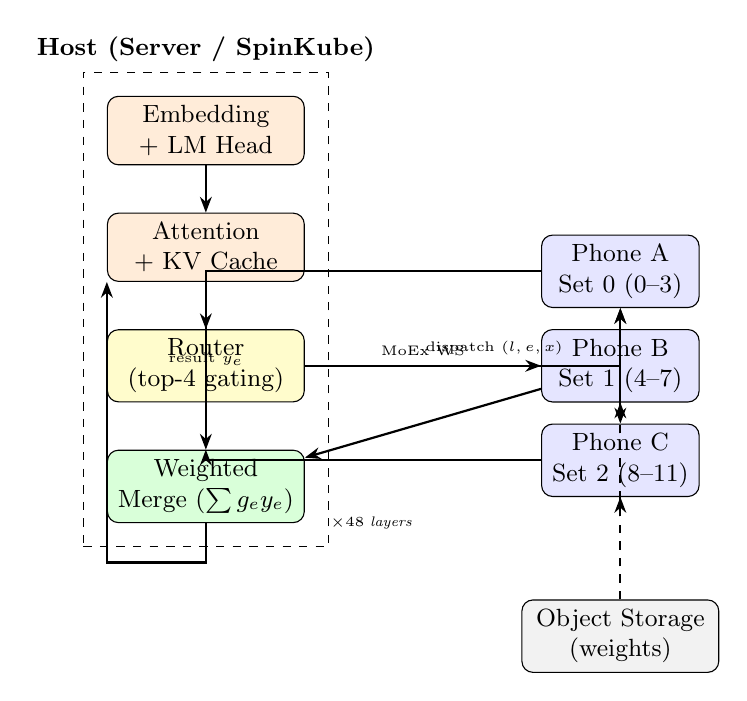
\begin{tikzpicture}[
  node distance=1.2cm and 1.5cm,
  box/.style={rectangle, draw, rounded corners, minimum width=2.5cm,
              minimum height=0.8cm, align=center, font=\small},
  phone/.style={rectangle, draw, rounded corners, minimum width=2cm,
                minimum height=0.8cm, fill=blue!10, align=center,
                font=\small},
  arr/.style={-{Stealth[length=2mm]}, thick},
  darr/.style={-{Stealth[length=2mm]}, thick, dashed},
]
  % Host
  \node[box, fill=orange!15] (emb) {Embedding\\+ LM Head};
  \node[box, fill=orange!15, below=0.6cm of emb] (attn) {Attention\\+ KV Cache};
  \node[box, fill=yellow!20, below=0.6cm of attn] (router) {Router\\(top-4 gating)};
  \node[box, fill=green!15, below=0.6cm of router] (merge) {Weighted\\Merge ($\sum g_e y_e$)};

  % Fit host
  \node[draw, dashed, fit=(emb)(attn)(router)(merge),
        inner sep=0.3cm, label={[font=\small\bfseries]above:Host (Server / SpinKube)}] (host) {};

  % Phones
  \node[phone, right=3cm of router, yshift=1.2cm] (p1) {Phone A\\Set 0 (0--3)};
  \node[phone, right=3cm of router] (p2) {Phone B\\Set 1 (4--7)};
  \node[phone, right=3cm of router, yshift=-1.2cm] (p3) {Phone C\\Set 2 (8--11)};

  % Blob
  \node[box, fill=gray!10, below=2.5cm of p2] (blob) {Object Storage\\(weights)};

  % Arrows
  \draw[arr] (emb) -- (attn);
  \draw[arr] (attn) -- (router);
  \draw[arr] (router) -| node[above, font=\tiny, pos=0.3]
    {dispatch $(l, e, x)$} (p1);
  \draw[arr] (router) -- node[above, font=\tiny] {MoEx WS} (p2);
  \draw[arr] (router) -| (p3);
  \draw[arr] (p1) -| node[below, font=\tiny, pos=0.7]
    {result $y_e$} (merge);
  \draw[arr] (p2) -- (merge);
  \draw[arr] (p3) -| (merge);
  \draw[arr] (merge.south) -- ++(0,-0.5) -| (attn.south west);

  % Blob arrows
  \draw[darr] (blob) -- (p1);
  \draw[darr] (blob) -- (p2);
  \draw[darr] (blob) -- (p3);

  % Layer loop annotation
  \node[font=\tiny\itshape, right=0.2cm of merge.south east] {$\times 48$ layers};
\end{tikzpicture}
\caption{MoEx system architecture. The host runs Attention + Router on
the server. Expert FFN computations are dispatched to phone workers
via WebSocket. Weights are loaded from object storage at registration
time.}
\label{fig:arch}
\end{figure}

Figure~\ref{fig:arch} shows the high-level architecture. The system
comprises three components:

\begin{enumerate}
  \item \textbf{Control Plane} (TinyGo SpinApp): Runs the
    host-side inference pipeline, device registry, dispatch
    orchestration, and MCP tool interface. Deployed at
    \texttt{1.etzhayyim.com/api/mcp}.

  \item \textbf{Expert Worker} (SvelteKit PWA): Runs on phones/browsers,
    initializes WebGPU, loads expert weights from object storage,
    connects to control plane via WebSocket, and executes dispatched
    FFN computations.

  \item \textbf{Weight Store} (Linode Object Storage): Hosts int4-quantized
    expert weight bundles ($\sim$480\,MB per 4-expert set) and host
    attention/router weights ($\sim$2.4\,GB).
\end{enumerate}

\subsection{Weight Decomposition}
\label{sec:decomp}

We decompose the Qwen3-30B-A3B checkpoint into:

\textbf{Host package} ($\sim$2.4\,GB):
\begin{itemize}
  \item Token embedding and LM head ($d_h = 2048$, vocab $\sim$151K)
  \item Per-layer: LayerNorm, QKV projection, attention output
    projection, router weights $W_r \in \mathbb{R}^{128 \times 2048}$
  \item KV cache (dynamic, per-request)
\end{itemize}

\textbf{Expert sets} (32 sets $\times$ $\sim$480\,MB each):
\begin{itemize}
  \item Each set contains 4 consecutive experts across all 48 layers
  \item Per expert per layer: $W_{\text{gate}}^e$, $W_{\text{up}}^e$
    ($768 \times 2048$ each), $W_{\text{down}}^e$ ($2048 \times 768$)
  \item Quantized to int4 with per-channel scale/zero-point
  \item Set $s$ covers experts $\{4s, 4s{+}1, 4s{+}2, 4s{+}3\}$
\end{itemize}

The total expert storage is $32 \times 480 = 15360$\,MB (int4). Each
device downloads one set at registration time.

\subsection{Device Registry and Scoring}

The control plane maintains a registry of active devices, indexed by
expert set ID. Each device tracks:

\begin{itemize}
  \item \textbf{RTT EMA} (exponential moving average, $\alpha = 0.3$)
  \item \textbf{Temperature} (reported by device, for thermal
    throttling awareness)
  \item \textbf{Foreground status} (apps in background may be
    throttled)
  \item \textbf{Job success/failure counts}
\end{itemize}

Device scoring for dispatch:
\begin{equation}
  \text{score}(d) = 0.4 \cdot \text{RTT}_d + 0.3 \cdot T_d \cdot 100
    + 0.3 \cdot \text{failrate}_d \cdot 1000 + \mathbb{1}[\neg\text{fg}] \cdot 50
  \label{eq:score}
\end{equation}
Lower score is better. The dispatcher selects the device with the
lowest score for each expert set.

% ============================================================
\section{MoEx Binary Protocol}
\label{sec:protocol}

Existing WebSocket framing for JSON-RPC adds 100--500 bytes of
overhead per message. For Expert FFN dispatch, each message carries
$2048 \times 4 = 8192$ bytes of float32 payload. We design a compact
binary protocol to minimize framing overhead.

\subsection{Wire Format}

\begin{table}[h]
\centering
\caption{MoEx message header (12 bytes, little-endian)}
\label{tab:header}
\begin{tabular}{@{}lccl@{}}
\toprule
Field & Offset & Size & Description \\
\midrule
Magic & 0 & 4B & \texttt{0x4D6F4578} (``MoEx'') \\
Type & 4 & 1B & Message type (see Table~\ref{tab:types}) \\
Layer ID & 5 & 1B & Transformer layer index (0--47) \\
Expert ID & 6 & 2B & Expert index (0--127) \\
Payload Len & 8 & 4B & Payload length in bytes \\
\bottomrule
\end{tabular}
\end{table}

\begin{table}[h]
\centering
\caption{Message types}
\label{tab:types}
\begin{tabular}{@{}ccl@{}}
\toprule
Code & Name & Direction \\
\midrule
\texttt{0x01} & \textsc{dispatch} & Host $\to$ Device \\
\texttt{0x02} & \textsc{result} & Device $\to$ Host \\
\texttt{0x03} & \textsc{hedge} & Host $\to$ Device (duplicate) \\
\texttt{0x04} & \textsc{ack} & Host $\to$ Device (cancel) \\
\texttt{0x10} & \textsc{register} & Device $\to$ Host \\
\texttt{0x11} & \textsc{heartbeat} & Bidirectional \\
\texttt{0x12} & \textsc{manifest} & Host $\to$ Device \\
\bottomrule
\end{tabular}
\end{table}

\subsection{Dispatch Payload}

A \textsc{dispatch} message payload contains:
\begin{itemize}
  \item Job ID (2-byte length prefix + UTF-8 string)
  \item Input hidden state ($d_h = 2048$ float32 values, 8192 bytes)
\end{itemize}

Total message size: $12 + 2 + |\text{job\_id}| + 8192 \approx 8.2$\,KB.

A \textsc{result} message payload contains:
\begin{itemize}
  \item Job ID (2-byte length prefix + UTF-8 string)
  \item Elapsed time (4-byte uint32, milliseconds)
  \item Output hidden state ($d_h = 2048$ float32 values, 8192 bytes)
\end{itemize}

% ============================================================
\section{Hedged Dispatch Strategy}
\label{sec:hedge}

\begin{algorithm}[t]
\caption{Hedged Expert Dispatch}
\label{alg:hedge}
\begin{algorithmic}[1]
\Require Layer $l$, expert ID $e$, input $x \in \mathbb{R}^{d_h}$
\Ensure Expert output $y_e \in \mathbb{R}^{d_h}$
\State $s \gets e \div 4$ \Comment{Expert set ID}
\State $d_1 \gets \text{BestDevice}(s)$
\State Send \textsc{dispatch}$(l, e, x)$ to $d_1$
\State $t_0 \gets \text{now}()$
\While{$\text{now}() - t_0 < 500\text{ms}$}
  \If{result received from any device}
    \State Send \textsc{ack} to other devices \Comment{Cancel hedge}
    \State \Return result
  \EndIf
  \If{$\text{now}() - t_0 \geq 50\text{ms}$ and not hedged}
    \State $d_2 \gets \text{AltDevice}(s, \text{exclude}=d_1)$
    \State Send \textsc{hedge}$(l, e, x)$ to $d_2$
    \Comment{Speculative duplicate}
  \EndIf
  \If{$\text{now}() - t_0 \geq 200\text{ms}$ and not resent}
    \State $d_3 \gets \text{AltDevice}(s, \text{exclude}=\{d_1,d_2\})$
    \State Send \textsc{dispatch}$(l, e, x)$ to $d_3$
    \Comment{Resend to fresh device}
  \EndIf
\EndWhile
\State \Return \textsc{timeout\_error}
\end{algorithmic}
\end{algorithm}

Algorithm~\ref{alg:hedge} describes the three-tier dispatch strategy.
The timeouts are chosen based on empirical mobile WebGPU latency
distributions:

\begin{itemize}
  \item \textbf{50\,ms hedge}: The p50 compute time for a single
    Expert FFN on a mid-range phone GPU is $\sim$30\,ms. Hedging at
    50\,ms catches devices that are slower than expected without
    wasting bandwidth on fast completions.

  \item \textbf{200\,ms resend}: Network jitter on cellular connections
    can add 50--150\,ms. Resending to a different device in the same
    set after 200\,ms handles network-level failures.

  \item \textbf{500\,ms fail}: Hard timeout. If no device in the set
    responds within 500\,ms, the dispatch fails and the layer is
    marked as degraded.
\end{itemize}

With a redundancy factor of 4 devices per set (across 100+ total
devices), the probability of all 4 devices failing within 500\,ms is
negligible under normal conditions.

% ============================================================
\section{WebGPU Expert Engine}
\label{sec:webgpu}

\subsection{Compute Shader Design}

We implement two WGSL compute shaders:

\textbf{GEMM kernel}: General matrix multiplication with workgroup
size $16 \times 16$:
\begin{lstlisting}[language=C, caption={GEMM compute shader (WGSL)}]
@compute @workgroup_size(16, 16)
fn main(@builtin(global_invocation_id) gid: vec3<u32>) {
  let row = gid.x; let col = gid.y;
  if (row >= M || col >= N) { return; }
  var sum: f32 = 0.0;
  for (var k: u32 = 0u; k < K; k++) {
    sum += A[row*K + k] * B[k*N + col];
  }
  C[row*N + col] = sum;
}
\end{lstlisting}

\textbf{SiLU$\odot$mul kernel}: Fused SiLU activation and
element-wise multiplication with workgroup size 256:
\begin{lstlisting}[language=C, caption={SiLU-mul compute shader (WGSL)}]
@compute @workgroup_size(256)
fn main(@builtin(global_invocation_id) gid: vec3<u32>) {
  let i = gid.x;
  if (i >= len) { return; }
  let silu = gate[i] / (1.0 + exp(-gate[i]));
  out[i] = silu * up[i];
}
\end{lstlisting}

\subsection{Expert FFN Pipeline}

For each dispatch, the engine executes:
\begin{enumerate}
  \item \textbf{Gate projection}: $g = W_{\text{gate}}^e \cdot x$
    (GEMM: $768 \times 2048 \times 1$)
  \item \textbf{Up projection}: $u = W_{\text{up}}^e \cdot x$
    (GEMM: $768 \times 2048 \times 1$)
  \item \textbf{SiLU-mul}: $a = \text{SiLU}(g) \odot u$
    (element-wise, 768 elements)
  \item \textbf{Down projection}: $y = W_{\text{down}}^e \cdot a$
    (GEMM: $2048 \times 768 \times 1$)
\end{enumerate}

Total FLOPs per expert: $2 \times (768 \times 2048) + 2 \times 768 +
2 \times (2048 \times 768) = 6,293,504 \approx 6.3$\,MFLOPS.

\subsection{Memory Requirements}

Per expert, per layer (fp32 after dequantization):
\begin{align*}
  W_{\text{gate}} &: 768 \times 2048 \times 4 = 6.0\text{\,MB} \\
  W_{\text{up}} &: 768 \times 2048 \times 4 = 6.0\text{\,MB} \\
  W_{\text{down}} &: 2048 \times 768 \times 4 = 6.0\text{\,MB}
\end{align*}

Per expert across 48 layers: $3 \times 6.0 \times 48 = 864$\,MB (fp32)
or $\sim$216\,MB (int4 storage, fp32 GPU buffers created on demand per
layer).

Per 4-expert set: $4 \times 216 \approx 864$\,MB (int4 storage), but
only one layer's buffers ($4 \times 18 = 72$\,MB fp32) need to reside
on GPU simultaneously.

\subsection{Browser Compatibility}

\begin{table}[h]
\centering
\caption{WebGPU compute shader support on mobile browsers}
\label{tab:compat}
\begin{tabular}{@{}llcc@{}}
\toprule
Platform & Browser & Compute & Max Buffer \\
\midrule
iOS 18+ & Safari & Yes & 256\,MB \\
Android 14+ & Chrome 121+ & Yes & 256\,MB \\
macOS 14+ & Safari/Chrome & Yes & 512\,MB \\
Windows 11 & Chrome/Edge & Yes & 256\,MB \\
\bottomrule
\end{tabular}
\end{table}

% ============================================================
\section{Latency Analysis}
\label{sec:latency}

The end-to-end latency for processing one token through one MoE layer
is:
\begin{equation}
  T_{\text{layer}} = T_{\text{attn}} + T_{\text{route}} +
    \max_{e \in \text{top-}k}
    \left(T_{\text{net}}^e + T_{\text{compute}}^e\right) +
    T_{\text{merge}}
  \label{eq:latency}
\end{equation}

\begin{table}[h]
\centering
\caption{Estimated latency budget per MoE layer}
\label{tab:latency}
\begin{tabular}{@{}lrl@{}}
\toprule
Component & Estimate & Notes \\
\midrule
$T_{\text{attn}}$ & 2--5\,ms & Server GPU, batch=1 \\
$T_{\text{route}}$ & $<$0.1\,ms & Small matmul ($128 \times 2048$) \\
$T_{\text{net}}$ (RTT) & 10--50\,ms & WiFi/LTE, WebSocket \\
$T_{\text{compute}}$ & 5--30\,ms & Mobile WebGPU, fp32 GEMM \\
$T_{\text{merge}}$ & $<$0.1\,ms & Weighted sum of 4 vectors \\
\midrule
\textbf{Total (p50)} & \textbf{20--40\,ms} & Per layer \\
\textbf{Total (48 layers)} & \textbf{1.0--1.9\,s} & Per token \\
\bottomrule
\end{tabular}
\end{table}

The dominant cost is network RTT, not compute. With hedged dispatch,
p99 latency improves by 2--3$\times$ compared to non-hedged dispatch,
as tail-latency events on individual devices are masked by the hedge.

\textbf{Pipeline parallelism opportunity}: Since the host processes
layers sequentially, and each layer's expert dispatch is independent,
the host can begin computing attention for layer $l+1$ while waiting
for expert results from layer $l$. This is feasible only if KV cache
updates from layer $l$'s attention are available before layer $l+1$
starts, which they are by construction.

% ============================================================
\section{Weight Distribution}
\label{sec:weights}

Expert weight sets are stored in Linode Object Storage
(\texttt{etzhayyim-static-sites} bucket, \texttt{jp-osa-1} region) and
served over HTTPS. The control plane provides a weight manifest via
MCP tool (\texttt{moe.get\_weight\_manifest}) containing:

\begin{itemize}
  \item Blob key (S3 path) for each set
  \item Size in MB
  \item SHA-256 checksum
  \item Expert IDs covered
\end{itemize}

The weight bundle format uses a simple header-then-tensors layout:
\begin{enumerate}
  \item 4-byte header length (uint32, little-endian)
  \item JSON header: tensor metadata (layer, expert, name, offset, length)
  \item Binary tensor data (int4 quantized, dequantized to fp32 on device)
\end{enumerate}

The control plane uses a \texttt{wasi:blobstore}
provider~\cite{wasiblobstore} to serve weights directly from S3,
enabling the blobstore capability to be swapped between providers
(S3, filesystem, Azure Blob) without component changes.

% ============================================================
\section{Governance: Compute Credits (GCC)}
\label{sec:gcc}

Expert computation is compensated via \textbf{Governance Compute
Credits (GCC)}, an ERC-20 token deployed on Ethereum mainnet:

\begin{itemize}
  \item GCC Token: \texttt{0x799d...F30B} (FiatTokenV2\_2, 6 decimals)
  \item GCCMinter: \texttt{0xAf80...F3d9} (accepts ETH/USDC/USDT)
  \item Safe multisig: \texttt{0xA003...F4E} (2/3 threshold)
\end{itemize}

Workers earn GCC proportional to jobs completed. An auction-based
assignment model (bid in GCC, penalty for failure) is planned but not
yet implemented. A 2\% random audit rate verifies computation
correctness by re-executing the same input on a trusted device and
comparing outputs.

% ============================================================
\section{Implementation}
\label{sec:impl}

\subsection{Control Plane (SpinKube)}

The control plane is implemented as a TinyGo SpinApp component
(\texttt{wasm/control-plane-25primzm/}) exposing MCP JSON-RPC 2.0
tools:

\begin{itemize}
  \item \texttt{moe.register\_device}: Register a device with set ID
  \item \texttt{moe.dispatch\_expert}: Dispatch FFN job to best device
  \item \texttt{moe.submit\_expert\_result}: Accept FFN result, update
    RTT EMA
  \item \texttt{moe.get\_network\_status}: Device count, set coverage,
    metrics
  \item \texttt{moe.get\_weight\_manifest}: Blob keys for weight download
  \item \texttt{moe.list\_devices}: All registered devices with scores
\end{itemize}

The component uses the \texttt{wasi:blobstore/blobstore@0.2.0-draft}
interface to access Linode Object Storage via the S3 blobstore
provider.

\subsection{Expert Worker (SvelteKit PWA)}

The expert worker (\texttt{cdn/expert-worker-5i9ktcbs/}) is a
SvelteKit static site with:

\begin{itemize}
  \item \texttt{expert-engine.ts}: WebGPU initialization, WGSL shader
    compilation, weight loading, SwiGLU FFN execution
  \item \texttt{transport.ts}: MoEx binary protocol
    encoder/decoder, \texttt{ExpertTransport} WebSocket client
  \item \texttt{+page.svelte}: UI for device configuration, worker
    status, job statistics
\end{itemize}

\subsection{Host Integration (Tauri)}

The host-side inference pipeline integrates with the Etzhayyim OS Tauri
desktop application (\texttt{projects/etzhayyim-project-os/}). The
Tauri app embeds a WebView that can run the control plane client,
providing a native desktop experience for orchestrating distributed
inference.

% ============================================================
\section{Discussion and Limitations}
\label{sec:discussion}

\textbf{Latency vs.\ throughput}: MoEx optimizes for \emph{throughput}
(tokens per second across many concurrent requests) rather than
single-request \emph{latency}. At 1--2 seconds per token, MoEx is
not competitive with server-only inference for interactive chat.
However, for batch workloads, the aggregate throughput of 100+ phone
GPUs can exceed a single server GPU.

\textbf{Network reliability}: Cellular networks exhibit high variance
in RTT. Hedged dispatch mitigates this, but sustained network
degradation across all devices in a set will cause failures. Set
replication (same experts on multiple devices) provides redundancy.

\textbf{Thermal throttling}: Phone GPUs throttle under sustained load.
The device scoring model penalizes high temperatures, but sustained
inference workloads will cause progressive performance degradation.
Short duty cycles (e.g., 5 minutes on, 5 minutes off) may be
necessary.

\textbf{Security}: A malicious worker could return incorrect results.
The 2\% audit rate provides probabilistic detection, and GCC penalties
disincentivize cheating. Deterministic verification (running the same
computation on two devices and comparing) is possible but doubles
compute cost.

\textbf{Weight piracy}: Distributing model weights to untrusted devices
raises IP concerns. Int4 quantization and per-expert granularity
limit the utility of stolen weights (a single 4-expert set cannot
perform full inference). Encryption-at-rest with per-session keys
is a potential mitigation.

% ============================================================
\section{Conclusion}
\label{sec:conclusion}

We presented MoEx, a system for distributed MoE inference that
disaggregates Expert FFN computation to consumer devices via WebGPU.
By exploiting the sparse activation pattern of MoE models, we reduce
per-device memory requirements to $\sim$480\,MB (4-expert set,
int4) and per-dispatch compute to $\sim$6.3\,MFLOPS, both well within
the capabilities of modern smartphones. The MoEx binary protocol
minimizes communication overhead, and hedged dispatch with device
scoring manages the inherent unreliability of consumer networks.

The system is fully implemented on SpinKube (control plane),
SvelteKit + WebGPU (expert worker), and Linode Object Storage
(weight distribution), with GCC ERC-20 tokens for compute
compensation. While single-token latency (1--2 seconds) limits
interactive use, the aggregate throughput of a fleet of phone GPUs
represents a novel compute resource for batch LLM inference.

\textbf{Future work} includes: (1) TVM/MLC compilation of the Expert
FFN module for optimized WebGPU kernels, (2) pipeline parallelism
between layers, (3) KV cache compression for reduced host memory,
(4) extension to other MoE models (Mixtral, DeepSeek-V3), and
(5) formal verification of the hedged dispatch protocol.

% ============================================================
\bibliographystyle{plainnat}

\begin{thebibliography}{20}

\bibitem[Borzunov et~al.(2023)]{borzunov2023petals}
Alexander Borzunov, Dmitry Baranchuk, Tim Dettmers, Max Ryabinin,
Younes Belkada, Artem Chumachenko, Pavel Samygin, and Colin Raffel.
\newblock Petals: Collaborative inference and fine-tuning of large
  models.
\newblock In \emph{Proceedings of the 61st ACL: System Demonstrations},
  2023.

\bibitem[Chen et~al.(2018)]{chen2018tvm}
Tianqi Chen, Thierry Moreau, Ziheng Jiang, Lianmin Zheng, Eddie Yan,
Meghan Cowan, Haichen Shen, Leyuan Wang, Yuwei Hu, Luis Ceze, Carlos
Guestrin, and Arvind Krishnamurthy.
\newblock TVM: An automated end-to-end optimizing compiler for deep
  learning.
\newblock In \emph{OSDI}, 2018.

\bibitem[Dean and Barroso(2013)]{dean2013tail}
Jeffrey Dean and Luiz Andr{\'e} Barroso.
\newblock The tail at scale.
\newblock \emph{Communications of the ACM}, 56(2):74--80, 2013.

\bibitem[Fedus et~al.(2022)]{fedus2022switch}
William Fedus, Barret Zoph, and Noam Shazeer.
\newblock Switch transformers: Scaling to trillion parameter models with
  simple and efficient sparsity.
\newblock \emph{JMLR}, 23(120):1--39, 2022.

\bibitem[Huang et~al.(2019)]{huang2019gpipe}
Yanping Huang, Youlong Cheng, Ankur Bapna, Orhan Firat, Mia~Xu Chen,
Dehao Chen, HyoukJoong Lee, Jiquan Ngiam, Quoc~V. Le, Yonghui Wu, and
Zhifeng Chen.
\newblock GPipe: Efficient training of giant neural networks using
  pipeline parallelism.
\newblock In \emph{NeurIPS}, 2019.

\bibitem[Lepikhin et~al.(2020)]{lepikhin2020gshard}
Dmitry Lepikhin, HyoukJoong Lee, Yuanzhong Xu, Dehao Chen, Orhan
Firat, Yanping Huang, Maxim Krikun, Noam Shazeer, and Zhifeng Chen.
\newblock GShard: Scaling giant models with conditional computation and
  automatic sharding.
\newblock In \emph{ICLR}, 2020.

\bibitem[{MLC-LLM Team}(2024)]{mlcllm2024}
{MLC-LLM Team}.
\newblock MLC LLM: Universal deployment of large language models.
\newblock \url{https://llm.mlc.ai/}, 2024.

\bibitem[{Qwen Team}(2025)]{qwen3}
{Qwen Team}.
\newblock Qwen3 technical report.
\newblock \url{https://qwenlm.github.io/blog/qwen3/}, 2025.

\bibitem[Shazeer(2020)]{shazeer2020glu}
Noam Shazeer.
\newblock GLU variants improve transformer.
\newblock \emph{arXiv:2002.05202}, 2020.

\bibitem[Shazeer et~al.(2017)]{shazeer2017outrageously}
Noam Shazeer, Azalia Mirhoseini, Krzysztof Maziarz, Andy Davis,
Quoc Le, Geoffrey Hinton, and Jeff Dean.
\newblock Outrageously large neural networks: The sparsely-gated
  mixture-of-experts layer.
\newblock In \emph{ICLR}, 2017.

\bibitem[Shoeybi et~al.(2019)]{shoeybi2019megatron}
Mohammad Shoeybi, Mostofa Patwary, Raul Puri, Patrick LeGresley, Jared
Casper, and Bryan Catanzaro.
\newblock Megatron-LM: Training multi-billion parameter language models
  using model parallelism.
\newblock \emph{arXiv:1909.08053}, 2019.

\bibitem[{W3C}(2024)]{webgpu2024}
{W3C}.
\newblock WebGPU specification.
\newblock \url{https://www.w3.org/TR/webgpu/}, 2024.

\bibitem[{WebLLM Team}(2024)]{webllm2024}
{WebLLM Team}.
\newblock WebLLM: High-performance in-browser LLM inference engine.
\newblock \url{https://webllm.mlc.ai/}, 2024.

\bibitem[{WASI}(2024)]{wasiblobstore}
{WASI Cloud}.
\newblock wasi-blobstore: Blob storage interface for WebAssembly.
\newblock \url{https://github.com/WebAssembly/wasi-blobstore}, 2024.

\end{thebibliography}

% ============================================================
\appendix
\section{MoEx Protocol Reference}
\label{app:protocol}

\begin{table}[h]
\centering
\caption{Complete MoEx message type registry}
\begin{tabular}{@{}cllp{6cm}@{}}
\toprule
Code & Name & Direction & Payload \\
\midrule
\texttt{0x01} & dispatch & H$\to$D & job\_id + float32[2048] \\
\texttt{0x02} & result & D$\to$H & job\_id + elapsed\_ms + float32[2048] \\
\texttt{0x03} & hedge & H$\to$D & Same as dispatch (speculative) \\
\texttt{0x04} & ack & H$\to$D & job\_id (cancel after first result) \\
\texttt{0x10} & register & D$\to$H & JSON \{device\_id, set\_id, gpu\} \\
\texttt{0x11} & heartbeat & Both & Empty \\
\texttt{0x12} & manifest & H$\to$D & JSON weight manifest \\
\bottomrule
\end{tabular}
\end{table}

\section{Expert Set Assignment}
\label{app:sets}

\begin{table}[h]
\centering
\caption{Expert set layout (Qwen3-30B-A3B, 128 experts, 32 sets)}
\begin{tabular}{@{}cccc@{}}
\toprule
Set ID & Expert IDs & Blob Key & Size (int4) \\
\midrule
0 & 0, 1, 2, 3 & \texttt{set-000.bin} & 480\,MB \\
1 & 4, 5, 6, 7 & \texttt{set-001.bin} & 480\,MB \\
$\vdots$ & $\vdots$ & $\vdots$ & $\vdots$ \\
31 & 124, 125, 126, 127 & \texttt{set-031.bin} & 480\,MB \\
\midrule
\multicolumn{3}{@{}l}{Total} & 15,360\,MB \\
\bottomrule
\end{tabular}
\end{table}

\end{document}
